\documentclass[11pt]{amsart}          
\usepackage[a4paper,verbose]{geometry}
\geometry{top=3cm,bottom=3cm,left=3cm,right=3cm,textheight=595pt}
\setlength{\parskip}{0.3em}
% ==============================
% PACKAGES
% ==============================

\usepackage{amsfonts}
\usepackage{amssymb}  
\usepackage{amsthm} 
\usepackage{amsmath} 
\usepackage{caption}
\usepackage[inline]{enumitem}
\setlist{itemsep=0em, topsep=0em, parsep=0em}
\setlist[enumerate]{label=(\alph*)}
\usepackage{etoolbox}
\usepackage{stmaryrd} 
\usepackage[dvipsnames]{xcolor}
\usepackage[]{hyperref}
\hypersetup{
  colorlinks,
  linkcolor=blue,
  citecolor=blue,
  urlcolor=blue}
\usepackage{graphicx}
\graphicspath{{assets/}}
\usepackage{mathtools}

\usepackage{tikz-cd}
\usepackage{minted}
\usepackage{float}
\usetikzlibrary{
  matrix,
  arrows,
  shapes
}

\setcounter{tocdepth}{1} % Sets depth for table of contents. 

\newcommand{\rr}{{\mathbb{R}}}
\newcommand{\nn}{{\mathbb{N}}}
\newcommand{\iso}{\cong}
\newcommand{\too}{\longrightarrow}
\newcommand{\tto}{\rightrightarrows}
\newcommand{\To}[1]{\xrightarrow{#1}}
\newcommand{\Too}[1]{\To{\;\;#1\;\;}}
\newcommand{\from}{\leftarrow}
\newcommand{\From}[1]{\xleftarrow{#1}}
\newcommand{\Cat}[1]{\mathbf{#1}}
\newcommand{\cat}[1]{\mathcal{#1}}
\newtheorem*{remark}{Remark}
\renewcommand{\ss}{\subseteq}
\newcommand{\hask}[1]{\mintinline{Haskell}{#1}}
\newenvironment{haskell}
  {\VerbatimEnvironment
  	\begin{minted}[escapeinside=??, mathescape=true,frame=single, framesep=5pt, tabsize=1]{Haskell}}
  {\end{minted}}

\author{Bartosz Milewski}
\title{Adjoint Functor Theorem}

\begin{document}
\maketitle{}

One of the tropes of detective movies is the almost miraculous ability to reconstruct an image from a blurry photograph. You just scan the picture,  say "enhance!", and voila, the face of the suspect or the registration number of their car appear on your computer screen. 

\includegraphics{BladeRunner.jpeg}

With constant improvements in deep learning, we might eventually be getting there. But in category theory, we do this all the time. We recover lost information. The way we do it is based on the basic tenet of category theory: an object is defined by its interactions with the rest of the world. This is the basis of all universal constructions, the Yoneda lemma, Grothendieck fibration, Kan extensions, and practically everything else. 

An iconic example is the construction of the left adjoint to a given functor. 

Consider a functor $R$ from some category $\cat D$ to another category $\cat C$. A functor, in general, loses some data, so it's usually impossible to invert it. I produces a "blurry" image of $\cat C$ inside $\cat D$. Its left adjoint is a functor from $\cat C$ to $\cat D$ that attempts to reconstruct lost information, to the best of its ability. Often the functor $R$ is \emph{forgetful}, which usually means that it purposefully forgets some information. It's left adjoint is then called \emph{free}, because it freely ad-libs the forgotten information. 


Of course, this is not always possible, but under certain conditions such left adjoint exists. These conditions are spelled out in the Freyd General Adjoint Functor Theorem. 

To understand them, we have to talk a little about size issues. A lot of interesting categories are large. It means there are so many objects in the category that they don't even form a set. The category of all sets, for instance, is large (there is no set of all sets). It's also possible that morphisms between two objects don't form a set. A category in which objects form a set is called \emph{small}, and a category in which hom-sets are sets is called \emph{locally small}. A lot of complexities in Freyd's theorem are related to size issues, so it's important to precisely spell out all the assumptions.

We assume that the source of the functor $R$, the category $\cat D$, is locally small. It must also be small-complete, that is every small diagram in $\cat D$ must have a limit. (A small diagram is a functor from a small category.) The functor $R$ must preserve all small limits. 

If it weren't for size issues, this would be enough to guarantee the existence of the left adjoint functor $L$, and we'll sketch the proof for this simplified case. In the general case, there is one more condition, the Solution Set Condition, which we'll discuss later.

Here's the problem we are trying to solve. We have the functor $R$ that maps objects and morphisms from $\cat D$ to $\cat C$. We want to define another functor $L$ that goes in the opposite direction. We're not looking for an inverse, so we're not expecting the composition of this functor with $R$ to be identity, but we want it to be \emph{related} to identity by two natural transformations called unit and counit. Their components are, respectively:
\[ \eta_c : c \to R L c\]
\[\epsilon_d : L R d \to d \]
and, as long as they satisfy some additional triangle identities, they will establish the adjunction $L \dashv R$.

To define $L$, lets pick an object $c$ in $\cat C$ and try to propagate it back to $\cat D$. To do that, we have to gather as much information about $c$ as possible. We will then propagate all this information back to $\cat D$ and find an object in $\cat D$ that "looks the same." In a way, we have to create a hologram of $c$ and communicate it back to $\cat D$. All the information about $c$ is encoded in morphisms so, in order to generate our hologram, we'll gather all morphisms that originate in $c$. These morphisms form a category called the coslice category $c/C$. 

The objects in $c/C$ are pairs $(c', f \colon c \to c')$. These are all the arrows that emanate from $c$, indexed by their target objects $c'$. But what really defines the structure of this category are morphisms between objects. A morphism in $c/C$ from $(c', f)$ to $(c'', g)$ is a morphism $h \colon c' \to c''$ that makes the following triangle commute:

\begin{figure}[H]
\centering
 \begin{tikzcd}
  & c
  \arrow[ld, "f"']
  \arrow[rd, "g"]\\
  c'
  \arrow[rr, "h"]
  && c''
\end{tikzcd}
\end{figure}

We have complete information about $c$ encoded in the slice category, but we have no way to propagate it back to $\cat D$. This is because, in general, the image of $\cat D$ doesn't cover the whole of $\cat C$. Even more importantly, not all morphisms in the image of $\cat D$ have corresponding morphisms in $\cat D$. We have to scale down our expectations, and define a partial hologram that does not capture all the information about $c$, but that can be back-propagated to $\cat D$. Such partial hologram is called a comma category $c/R$.

The objects of $c/R$ are pairs $(d, f \colon c \to R d)$, where $d$ is an object in $\cat D$. These are all the arrows emanating from $c$ whose target is in the image of $R$. Again, the important structure is encoded in the morphisms of $c/R$. These are the arrows in $\cat D$, $h \colon d \to d'$ that make the following diagram commute in $\cat C$

\begin{figure}[H]
\centering
 \begin{tikzcd}
  & c
  \arrow[ld, "f"']
  \arrow[rd, "g"]\\
  R d
  \arrow[rr, "R h"]
  && R d'
\end{tikzcd}
\end{figure}
Notice an interesting fact: we can interpret these triangles as commutation conditions in a cone with a vertex $c$ and the base formed by a selection of objects and morphisms from the image of $R$. Not all objects and not all morphism in the image of $R$ are included. In fact, only the ones that satisfy the cone condition are selected. 

\begin{figure}[H]
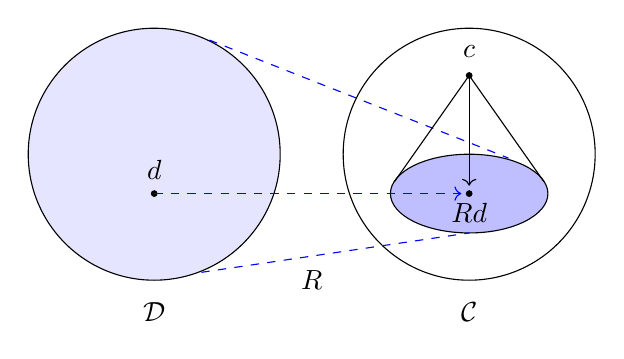
\begin{tikzpicture}
  \def\Xa{-2.0};
  \def\Xb{2.0};
  \def\Ytip{1.0};
  \def\Yo{-0.5};
  \def\Yb{-2.0};
         \draw (\Xa, 0)[fill=blue!10!white]  ellipse (1.6 and 1.6);
         \draw (\Xb , 0) ellipse (1.6 and 1.6);
         \draw (\Xb , \Yo)[fill=blue!25!white] ellipse (1 and 0.5);
         
        \filldraw (\Xb, \Ytip) circle (1pt);
        \node at ( \Xb, \Ytip + 0.3) { $c$ };
        
        \filldraw (\Xa, \Yo) circle (1pt);
        \node at ( \Xa, \Yo + 0.3) { $d$ };
        
        \filldraw (\Xb, \Yo) circle (1pt);
        \node at ( \Xb, \Yo - 0.25) { $R d$ };
	\draw[->, blue, dashed] (\Xa, \Yo) -- (\Xb - 0.1, \Yo);
	
	\draw[->] (\Xb, \Ytip) -- (\Xb, \Yo + 0.1);
        
        \node at (\Xa, \Yb) { $\cat D$ };
        \node at (\Xb, \Yb) { $\cat C$ };
        \node at (0, \Yb + 0.4) { $R$ };

	\draw [blue, dashed] (\Xa + 0.7, \Ytip + 0.45) -- (\Xb + 0.5, \Yo + 0.45);
	\draw [blue, dashed] (\Xa + 0.6, \Yo - 1) -- (\Xb, \Yo - 0.5);
	
	\draw (\Xb, \Ytip) -- (\Xb + 0.95, \Yo + 0.15);
	\draw (\Xb, \Ytip) -- (\Xb - 0.95, \Yo + 0.15);

\end{tikzpicture}
\end{figure}

We can now take all this information about $c$ that's been encoded in $c/R$ and move it back to $\cat D$. We define a projection functor $\pi_c \colon c/R \to D$ that maps $(d, f)$ to $d$, thus forgetting the morphism $f$. What's important, though, is that it keeps the information encoded in the morphisms of $c/R$, because these are just some morphisms in $\cat D$.

\begin{figure}[H]
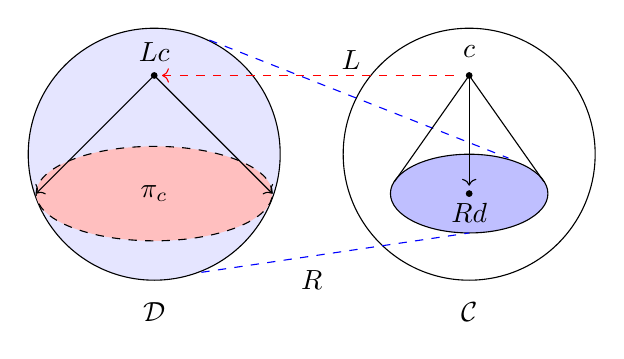
\begin{tikzpicture}
  \def\Xa{-2.0};
  \def\Xb{2.0};
  \def\Ytip{1.0};
  \def\Yo{-0.5};
  \def\Yb{-2.0};
         \draw (\Xa, 0)[fill=blue!10!white]  ellipse (1.6 and 1.6);
         \draw (\Xb , 0) ellipse (1.6 and 1.6);
         \draw (\Xb , \Yo)[fill=blue!25!white] ellipse (1 and 0.5);
         
        \filldraw (\Xb, \Ytip) circle (1pt);
        \node at ( \Xb, \Ytip + 0.3) { $c$ };
        
        \filldraw (\Xb, \Yo) circle (1pt);
        \node at ( \Xb, \Yo - 0.25) { $R d$ };
	
	\draw[->] (\Xb, \Ytip) -- (\Xb, \Yo + 0.1);
        
        \node at (\Xa, \Yb) { $\cat D$ };
        \node at (\Xb, \Yb) { $\cat C$ };
        \node at (0, \Yb + 0.4) { $R$ };

	\draw [blue, dashed] (\Xa + 0.7, \Ytip + 0.45) -- (\Xb + 0.5, \Yo + 0.45);
	\draw [blue, dashed] (\Xa + 0.6, \Yo - 1) -- (\Xb, \Yo - 0.5);
	
	\draw (\Xb, \Ytip) -- (\Xb + 0.95, \Yo + 0.15);
	\draw (\Xb, \Ytip) -- (\Xb - 0.95, \Yo + 0.15);

         \draw (\Xa , \Yo)[fill=red!25!white, dashed] ellipse (1.5 and 0.6);
         \node at (\Xa , \Yo) { $\pi_c$ };
	\draw[<-, red, dashed] (\Xa + 0.1, \Ytip) -- (\Xb - 0.1, \Ytip);
        \node at (0.5, \Ytip + 0.2) { $L$ };
        \filldraw (\Xa, \Ytip) circle (1pt);
        \node at (\Xa, \Ytip + 0.3) { $L c$ };

        \draw[->] (\Xa, \Ytip) -- (\Xa - 1.5, \Yo);
        \draw[->] (\Xa, \Ytip) -- (\Xa + 1.5, \Yo);
\end{tikzpicture}
\end{figure}

The image of $\pi_c$ doesn't necessarily cover the whole of $\cat D$, because not every $R d$ has arrows coming from $c$. Similarly, only the morphisms that make the appropriate triangle in $\cat C$ commute are picked by $\pi_c$. But those objects and morphisms that are in the image of $\pi_c$ form a diagram in $\cat C$. This diagram is our partial hologram and we can use it to pick an object in $\cat D$ that looks exactly like $c$. That object is the limit of this diagram. 

Here's the tricky part: we assumed that $\cat D$ is small-complete, so every small diagram has a limit, but the diagram defined by $\pi_c$ is not necessarily small. Let's ignore this problem for a moment, and proceed with sketching the proof that the mapping that assigns the limit of $\pi_c$ to every $c$ is the functor $L$ that is left adjoint to $R$. 

Let's see if we can define the unit
\[ \eta_c : c \to R L c\]
We have defined $L c$ as the limit of the diagram $\pi_c$. We also assumed that $R$ preserves limits (small limits, really; but let's ignore the size problems for the moment). That means that $R L c$ is the limit of the diagram $R \pi_c$ in $\cat C$. But, as we noticed before, this diagram is exactly the base of the cone with the apex $c$ that was used to define the comma category $c/R$. Since $R L c$ is the limit of this diagram, there is a unique morphism from any other cone to it. In particular there is a morphism from $c$ to it, and that's the morphism we'll chose for $\eta_c$. 

The component of the counit is a morphism
\[\epsilon_d : L R d \to d \]
We perform the construction starting with $c = R d$. We define the comma category $R d / R$ and use $\pi_{R d}$ to create the diagram whose limit is $L R d$. We pick $\epsilon_d$ to be a side of the limiting cone. We know that $d$ is in the base of the cone, because it's the projection of $(d, id \colon R d \to R d)$. 

To complete this proof, one should show that the unit and counit are natural transformations and that they satisfy triangle identities. 

So what about these pesky size issues? 

\end{document}


